\chapter{Risultati sperimentali}
\label{sec:risultati_sperimentali}

In questo capitolo vengono presentati e discussi i risultati sperimentali ottenuti 
attraverso una serie di test condotti sul progetto.
Il focus principale degli esperimenti è stato la valutazione dell'efficienza e della 
sicurezza delle due implementazioni dei crittosistemi discusse nelle sezioni precedenti. 
È importante sottolineare che questi test non si sono limitati ai singoli moduli 
crittografici, ma hanno considerato il progetto nella sua interezza, includendo tutte 
le sue componenti interconnesse attraverso il terzo modulo di supporto \texttt{Utils}.
Per fornire una valutazione completa, i risultati ottenuti sono stati confrontati con dati 
di test passati eseguiti da altri autori, ove disponibili. 
Questa comparazione ha permesso di esaminare i vantaggi e le limitazioni delle nuove 
implementazioni rispetto a soluzioni già note e testate.
Tutte le misurazioni sono state effettuate su una macchina con 16 GB di RAM e un processore 
Intel Core i5-11400F, con una frequenza operativa compresa tra 1.60 GHz e 4.40 GHz.
Per una maggiore chiarezza, in questo capitolo, il termine "GGH-HNF" farà sempre riferimento 
alla versione con \texttt{GGH\_private} impostato su \texttt{False}, salvo diversa indicazione.
I risultati presentati in ciascuna tabella, inoltre, utilizzano i punti al posto delle virgole come 
separatore decimale. Quindi, un valore come 792.555 rappresenta in realtà 
circa 793 secondi, non 792555. Questa convenzione di notazione è importante da 
tenere a mente quando si interpretano i dati, poiché influenza significativamente la 
lettura dei valori numerici.

\section{Generazione delle chiavi}
\label{sec:risultati_chiavi}

Per confrontare le prestazioni delle due implementazioni in termini di tempi di generazione 
e dimensioni delle chiavi, si è proceduto con la generazione di 10 coppie di chiavi 
(pubbliche e private) per ogni dimensione, partendo da 100 e aumentando di 100 unità alla volta 
fino a raggiungere 800. Tutti i parametri dei crittosistemi sono sono rimasti impostati 
sul default, fatta eccezione per \texttt{dimension} e \texttt{debug}, il primo usato per 
dettare la dimensione ad ogni iterazione e il secondo per effettuare il calcolo dei tempi
di ciascuno step. I tempi di generazione delle chiavi sono dati dalle seguenti formule:
\begin{itemize}
    \item Chiave privata:
    \begin{itemize}
        \item Per entrambi i crittosistemi è stato sufficiente calcolare il tempo di 
        generazione della base casuale (nel caso di GGH-HNF con riduzione LLL). Il tempo
        finale comprende anche il calcolo del determinante della matrice risultante 
        per verificarne l'invertibilità. Se una matrice generata non risulta essere 
        invertibile, l'iterazione viene rieseguita per non inquinare i risultati finali. 
    \end{itemize}
    \item Chiave pubblica:
    \begin{itemize}
        \item GGH: Il tempo di generazione della chiave pubblica è dato:
        $$\texttt{pubkey\_time} = \texttt{unim\_time}+\texttt{sigma\_time}+\texttt{pub\_time}$$
        dove: \texttt{unim\_time} è il tempo di generazione della matrice unimodulare, 
        \texttt{sigma\_time} è il tempo di generazione del sigma e \texttt{pub\_time} è il 
        tempo per effettuare il calcolo dell'Equazione \ref{eq:GGHencryption}.
        \item GGH-HNF: Il tempo di generazione della chiave pubblica è dato:
        $$\texttt{pubkey\_time} = \texttt{rho\_time}+\texttt{pub\_time}$$
        dove: \texttt{rho\_time} è il tempo di generazione del $\rho$ e 
        \texttt{pub\_time} è il tempo per effettuare il calcolo dell'Equazione \ref{eq:HNFencryption}.
    \end{itemize} 
\end{itemize}

\begin{table}[H]
    \centering
    \begin{tabular}{|c|c|c|c|c|}
        \hline
        \multirow{2}{*}{Dimensione} & 
        \multicolumn{2}{c|}{Tempo chiave privata (s)} & 
        \multicolumn{2}{c|}{Tempo chiave pubblica (s)} \\
        \cline{2-5}
        & GGH & GGH-HNF & GGH & GGH-HNF \\
        \hline
        100 & 0.009 & 0.030 & 0.491 & 0.063 \\
        200 & 0.046 & 0.187 & 3.626 & 0.213 \\
        300 & 0.111 & 0.618 & 12.991 & 0.618 \\
        400 & 0.234 & 0.927 & 34.056 & 1.444 \\
        500 & 0.411 & 1.676 & 74.576 & 2.728 \\
        600 & 0.930 & 2.747 & 184.469 & 6.065 \\
        700 & 1.107 & 5.484 & 251.482 & 14.525 \\
        800 & 1.546 & 5.942 & 368.591 & 22.277 \\
        \hline
    \end{tabular}
    \caption{Tempi medi di generazione delle chiavi di GGH e GGH-HNF.}
    \label{tab:key_gen_comparison}

\end{table}

\begin{table}[htbp]
    \centering
    \begin{tabular}{|c|c|c|c|c|}
        \hline
        \multirow{2}{*}{Dimensione} & 
        \multicolumn{2}{c|}{Dimensione chiave privata (KB)} & 
        \multicolumn{2}{c|}{Dimensione chiave pubblica (KB)} \\
        \cline{2-5}
        & GGH & GGH-HNF & GGH & GGH-HNF \\
        \hline
        100 & 24.862 & 34.615 & 97.656 & 44.611 \\
        200 & 98.580 & 156.392 & 677.253 & 195.580 \\
        300 & 221.042 & 366.645 & 2107.403 & 462.928 \\
        400 & 392.332 & 666.127 & 4936.998 & 851.883 \\
        500 & 612.420 & 1053.891 & 9481.981 & 1366.516 \\
        600 & 882.048 & 1529.102 & 16249.625  & 2009.303 \\
        700 & 1200.219 & 2093.324 & 25162.143 & 2782.517 \\
        800 & 1566.549 & 2744.888 & 36664.683 & 3688.281 \\
        \hline
    \end{tabular}
    \caption{Dimensioni medie delle chiavi di GGH e GGH-HNF.}
    \label{tab:key_size_comparison}
\end{table}

Analizzando i risultati complessivi riportati nelle Tabelle \ref{tab:key_gen_comparison} e 
\ref{tab:key_size_comparison}, relative ai tempi di generazione 
in secondi e alle dimensioni in Kilobytes delle chiavi, emergono sostanziali differenze tra GGH e GGH-HNF.
Per quanto riguarda la chiave privata, GGH dimostra prestazioni leggermente superiori 
sia in termini di velocità di generazione che di dimensioni, con tempi e spazio di 
archiviazione consistentemente inferiori per tutte le dimensioni testate. Al contrario, 
GGH-HNF si distingue ampiamente nella gestione della chiave pubblica, superando di gran 
lunga GGH in entrambi gli aspetti. In particolare, i tempi di generazione della chiave 
pubblica per GGH-HNF sono significativamente più bassi (ad esempio, circa 22 secondi 
contro 368 secondi di GGH per una dimensione di 800), e le dimensioni delle chiavi 
pubbliche risultano notevolmente più contenute (circa 3.7 MB per GGH-HNF contro 36.7 MB 
per GGH, sempre per dimensione 800). I risultati confermano come la forma normale di 
Hermite sia nettamente migliore della controparte usata in GGH. 
Grazie alla sua struttura triangolare, metà della matrice è composta da zeri, 
il che comporta due vantaggi significativi quando viene impiegata come operatore: 
una riduzione delle dimensioni della matrice e una minore complessità computazionale.
La generazione della chiave pubblica nel sistema GGH è significativamente rallentata 
dal processo di inversione della chiave privata, necessario per il calcolo di $\sigma$. 
Come evidenziato in Tabella \ref{tab:ggh_pub_key_gen_times}, che illustra i tempi medi 
di generazione per ogni fase, questo passaggio costituisce una porzione considerevole 
del tempo totale richiesto per la generazione della chiave pubblica, circa il 62.53\%. 
Sebbene sia possibile eliminare il tempo di generazione di $\sigma$ impostando un valore 
prefissato per il parametro \texttt{sigma}, GGH-HNF rimane comunque più veloce. 
Come illustrato nella Tabella \ref{tab:ggh_hnf_pub_key_gen_times}, 
i tempi di generazione per GGH-HNF benché condizionati dal calcolo della forma normale di 
Hermite, risultano sorprendentemente inferiori a quello che ci si aspettava nel 
rispetto dei test eseguiti in \cite{HNF04}, rendendo la generazione 
complessivamente più veloce. Per quanto riguarda la chiave 
privata di GGH-HNF invece, è possibile affermare che il suo tempo di generazione medio è trascurabilmente
superiore a quello di GGH, con una differenza di circa 4 secondi in dimensione 800. Al contrario
la dimensione è maggiore di circa 1.1MB rendendola quindi di qualità inferiore rispetto alla
sua controparte. 
    
\begin{table}[H]
    \centering
    \begin{tabular}{|c|c|c|c|}
    \hline
    Dimensione & 
    \begin{tabular}[c]{@{}c@{}}Tempo medio\\Sigma (s)\end{tabular} & 
    \begin{tabular}[c]{@{}c@{}}Tempo medio\\Matrice Unimodulare $\mathbf{U}$ (s)\end{tabular} & 
    \begin{tabular}[c]{@{}c@{}}Tempo medio\\ Calcolo di $\mathbf{U}\times\mathbf{R}$ (s)\end{tabular} \\ 
    \hline
    100       & 0.181     & 0.310    & 0.001  \\ 
    200       & 1.845     & 1.768    & 0.013  \\ 
    300       & 7.817     & 5.113    & 0.061  \\ 
    400       & 21.459    & 12.460   & 0.137  \\ 
    500       & 49.384    & 24.937   & 0.255  \\ 
    600       & 129.887   & 53.991   & 0.592  \\
    700       & 185.891   & 64.772   & 0.819  \\ 
    800       & 368.591   & 97.709   & 1.372  \\ 
    \hline
    \end{tabular}
    \caption{Tempi medi di generazione degli step della chiave pubblica in GGH.}
    \label{tab:ggh_pub_key_gen_times}
\end{table}

\begin{table}[h]
        \centering
        \begin{tabular}{|c|c|c|}
        \hline
        Dimensione &
        \begin{tabular}[c]{@{}c@{}}Tempo medio\\Rho (s)\end{tabular} & 
        \begin{tabular}[c]{@{}c@{}}Tempo medio\\ HNF (s)\end{tabular} \\
        \hline
        100 & 0.043 & 0.021 \\
        200 & 0.193 & 0.213 \\
        300 & 0.471 & 0.713 \\
        400 & 0.927 & 1.444 \\
        500 & 1.676 & 2.728 \\
        600 & 2.747 & 6.065 \\
        700 & 5.484 & 14.525 \\
        800 & 5.942 & 16.335 \\
        \hline
        \end{tabular}
        \caption{Tempi medi di generazione degli step della chiave pubblica in GGH-HNF.}
        \label{tab:ggh_hnf_pub_key_gen_times}
\end{table}

Un'ulteriore proprietà che differenzia particolarmente i due metodi di generazione della 
chiave privata sta nel valore assunto da $\rho$, un parametro chiave che determina il 
successo della decifratura e la lunghezza assumibile dal vettore di errore. 
I dati relativi al cambiamento del $\rho$, in funzione della dimensione della chiave privata, riportati in 
Figura \ref{fig:rho_comparison}, sono stati raccolti durante un secondo esperimento, 
il quale sarà descritto dettagliatamente nella sezione successiva. 
È subito osservabile quanto il valore medio di $\rho$ cresca in maniera significativamente 
più rapida nel caso in cui \texttt{GGH\_private} sia impostato su \texttt{True} rispetto a 
\texttt{False}. In particolare, per dimensioni più grandi della chiave, come 800, si nota 
che il valore di $\rho$ supera i 9600 con \texttt{GGH\_private} $=$ \texttt{True}, mentre 
rimane intorno ai 600 con \texttt{GGH\_private} $=$ \texttt{False}. Le conseguenze di 
tali differenze drastiche, discusse più in dettaglio nella sezione successiva, è notabile 
in fase di decifratura e potrebbe essere altrettanto importante per la crittoanalisi. 

\begin{figure}[H]
    \centering
    \pgfplotsset{scaled y ticks=false}
    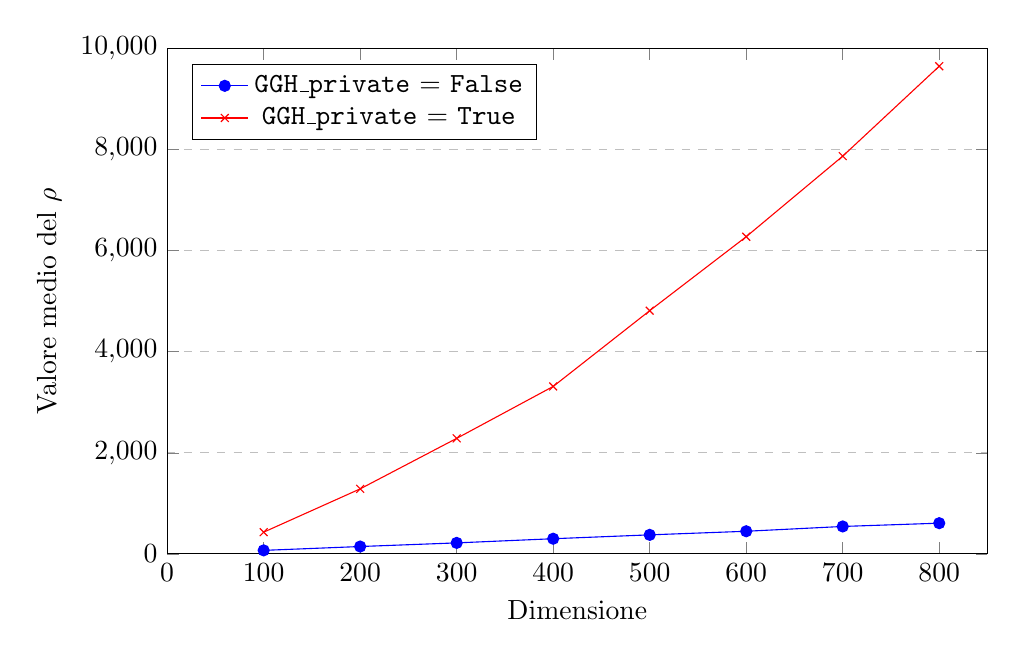
\begin{tikzpicture}
    \begin{axis}[
        width=12cm,
        height=8cm,
        xlabel={Dimensione},
        ylabel={Valore medio del $\rho$},
        xmin=0, xmax=850,
        ymin=0, ymax=10000,
        xtick={0,100,200,300,400,500,600,700,800},
        ytick={0,2000,4000,6000,8000,10000},
        legend pos=north west,
        ymajorgrids=true,
        grid style=dashed,
    ]

    \addplot[
        color=blue,
        mark=*,
        ]
        coordinates {
        (100,69.62374648610656)
        (200,145.76343496186707)
        (300,217.71290815546293)
        (400,300.14600247370022)
        (500,376.54398134961855)
        (600,447.74893878753156)
        (700,542.84539680420312)
        (800,607.85130753366593)
        };
        
    \addplot[
        color=red,
        mark=x,
        ]
        coordinates {
        (100,429.82235393365000)
        (200,1286.39891941831000)
        (300,2285.61614409605000)
        (400,3313.17114741192000)
        (500,4812.11168835805000)
        (600,6275.89251563181000)
        (700,7869.73987635605000)
        (800,9649.59255578677000)
        };
        
    \legend{\texttt{GGH\_private} = \texttt{False}, \texttt{GGH\_private} = \texttt{True}}

    \end{axis}
    \end{tikzpicture}
    \caption{Confronto del valore medio di $\rho$ con \texttt{GGH\_private} $=$ \texttt{True} o \texttt{False}.}
    \label{fig:rho_comparison}
\end{figure}


\section{Cifratura e decifratura}
\label{sec:risultati_cifratura_decifratura}

\begin{table}[htbp]
    \centering
    \begin{tabular}{|c|c|c|c|c|}
        \hline
        \multirow{2}{*}{Dimensione} & 
        \multicolumn{2}{c|}{Tempo di cifratura (s)} & 
        \multicolumn{2}{c|}{Tempo di decifratura (s)} \\
        \cline{2-5}
        & GGH & GGH-HNF & GGH & GGH-HNF \\
        \hline
        100 & $\approx$0 & 0.001 & 0.323 & 0.227 \\
        200 & $\approx$0 & 0.005 & 3.787 & 2.979 \\
        300 & 0.004 & 0.011 & 14.820 & 13.214 \\
        400 & 0.014 & 0.019 & 41.887 & 39.836 \\
        500 & 0.025 & 0.030 & 102.415 & 94.337 \\
        600 & 0.044 & 0.047 & 272.059 & 225.689 \\
        700 & 0.049 & 0.071 & 352.680 & 343.373 \\
        800 & 0.070 & 0.077 & 792.555 & 645.152 \\
        \hline
    \end{tabular}
    \caption{Tempi di cifratura e decifratura medi di GGH e GGH-HNF.}
    \label{tab:enc_dec_comparison}
\end{table}

L'esperimento illustrato all'inizio della sezione precedente, che ha analizzato le 
caratteristiche delle chiavi generate, è stato ulteriormente ampliato per includere una 
valutazione approfondita delle prestazioni dei processi di cifratura e decifratura. 
Oltre all'analisi delle chiavi, sono stati misurati i tempi medi di esecuzione, 
nonché calcolata la dimensione media del testo cifrato risultante. 
I risultati di queste misurazioni sono stati organizzati in due 
tabelle distinte: la Tabella \ref{tab:enc_dec_comparison} presenta i dati relativi ai 
tempi di esecuzione, mentre la Tabella \ref{tab:ciphertext_size_comparison} riporta le 
informazioni sulla grandezza del testo cifrato. 
Entrambi i crittosistemi mostrano tempi di cifratura significativamente più bassi rispetto
a quelli di decifratura. GGH presenta un lieve vantaggio in termini di velocità di 
cifratura, ma la differenza è minima. È da sottolineare il fatto che i tempi di cifratura 
rimangono contenuti, non superando 0.1 secondi anche per input di dimensioni considerevoli, il 
che evidenzia l'efficienza computazionale dei metodi di cifratura impiegati in entrambi gli schemi.
In fase di decifratura invece si osserva una crescita non lineare dei tempi all'aumentare 
della dimensione dell'input, con GGH-HNF che mostra generalmente prestazioni leggermente 
migliori rispetto a GGH, soprattutto per dimensioni maggiori. 
Questa differenza è attribuibile al fatto che GGH richiede l'inversione sia della base privata 
che di quella pubblica, mentre GGH-HNF necessita solo dell'inversione della base privata.
La notevole disparità temporale tra i processi di cifratura e decifratura è un fenomeno atteso. 
Questa differenza è principalmente dovuta alla necessità di invertire almeno una base durante 
la decifratura, un'operazione che richiede un considerevole sforzo computazionale. 

\begin{table}[htbp]
    \centering
    \begin{tabular}{|c|c|c|c|c|}
        \hline
        \multirow{2}{*}{Dimensione} & 
        \multicolumn{2}{c|}{Dimensione testo cifrato (KB)} \\
        \cline{2-3}
        & GGH & GGH-HNF\\
        \hline
        100 & 1.412  & 0.450  \\ 
        200 & 4.626  & 0.984  \\
        300 & 9.830  & 1.549  \\
        400 & 16.802 & 2.135 \\
        500 & 25.629 & 2.739  \\
        600 & 36.511 & 3.355  \\
        700 & 48.587 & 3.982  \\
        800 & 62.014 & 4.617  \\
        \hline
    \end{tabular}
    \caption{Dimensioni medie del testo cifrato di GGH e GGH-HNF.}
    \label{tab:ciphertext_size_comparison}
\end{table}

Spostando l'attenzione invece sulla dimensione del testo cifrato è immediatamente evidente 
che GGH-HNF superi notevolmente GGH in termini di efficienza spaziale.
GGH-HNF riesce a mantenere la dimensione del testo cifrato sotto i 5 KB, persino quando 
si lavora con una dimensione di 800. Al contrario, GGH produce un output significativamente 
più voluminoso, raggiungendo i 62 KB nelle stesse condizioni. 
Le motivazioni dietro questa diversità peculiare sta nella struttura intrinseca dei due 
testi cifrati. Osservando la Figura \ref{fig:ciphertexts_comparation}, che illustra i vettori 
rappresentanti i testi cifrati generati in dimensione 7 con parametri predefiniti, si nota che il 
testo cifrato di GGH-HNF, denominato $\mathbf{c}_{\text{HNF}}$, si compone della
maggior parte di numeri a singola cifra, 
seguiti infine da un unico numero intero di grande valore. Questa struttura è il risultato 
diretto dell'operazione modulare di $\mathbf{e}$ con la base pubblica in forma HNF, 
la cui particolare configurazione genera questo output compatto. In contrasto, 
il testo cifrato di GGH, $\mathbf{c}_{\text{GGH}}$, presenta una serie di numeri 
interi di media grandezza, sia positivi che negativi, distribuiti uniformemente 
nel vettore. La dimensione di questi valori è direttamente proporzionale alla grandezza
delle chiavi, portando il testo cifrato ad appesantirsi sempre di più con l'aumentare 
della dimensione. 

\begin{figure}[h!]
    \centering
    \texttt{$\mathbf{c}_{\text{HNF}} = $[0, 0, 0, 0, 0, 0, 2371763]}\\
    \texttt{$\mathbf{c}_{\text{GGH}} = $[6074, 1396, -137, 235, 842, -4540, -4766]}
    \caption{Comparazione fra le strutture dei testi cifrati di GGH e GGH-HNF.}
    \label{fig:ciphertexts_comparation}
\end{figure}

Nell'implementazione di GGH-HNF è stata data la possibilità all'utente di poter decidere
con quale metodo generare la chiave privata attraverso il parametro \texttt{GGH\_private}.
Come precedentemente accennato, è stato quindi svolto un secondo esperimento per valutare 
le conseguenze e i cambiamenti di tale scelta. Dal precedente test possiamo affermare
che il metodo di GGH genera matrici meno pesanti con meno tempo rispetto alla tecnica
usata da Micciancio. Ciò che non viene dimostrato è l'impatto in termini di percentuale 
di successo e sicurezza. Per valutare il secondo termine è stato svolto un ulteriore 
test specifico, descritto nella prossima sezione. 
Per quanto riguarda l'analisi dei successi, seguendo l'approccio del precedente esperimento,
sono state generate nuovamente 10 
coppie di chiavi pubbliche e private per ciascuna dimensione, 
partendo da 100 fino a 800, con incrementi di 100.
Tuttavia, per valutare l'efficacia di ciascun metodo di generazione della chiave privata, 
è stato introdotto il parametro \texttt{sigma}.
In questo nuovo test, per ogni dimensione e per ogni set di 10 
prove, sono stati applicati diversi valori del valore $\rho$, modulati da un fattore 
moltiplicativo determinato dal parametro \texttt{sigma}. 
I valori di \texttt{sigma} utilizzati erano compresi tra 0.50 e 1, con incrementi di 0.10. 
Complessivamente, sono state generate e analizzate 480 istanze del crittosistema, 
risultanti dalla combinazione di 10 test per ciascuna delle 8 dimensioni considerate e 
per ognuno dei 6 valori di \texttt{sigma}.
I risultati, osservabili in Tabella \ref{tab:combined_successes_hnf}, sono sorprendenti. 
Il metodo di GGH mostra una performance perfetta in tutte le dimensioni e per tutti i valori 
di \texttt{sigma}, con un tasso di successo del 100\% in ogni caso. Il metodo di 
Micciancio invece, seppur mostri generalmente buone prestazioni, soffre di alcune 
imperfezioni con un totale di 16 fallimenti sui 480 tentativi. Il fatto che il numero di errori
aumenti con l'aumentare di \texttt{sigma} non è una sorpresa: dato l'uso della
tecnica di arrotondamento di Babai per la decifratura, una scelta di lunghezza del 
vettore di errore troppo vicina al $\rho$ risulta in un aumento delle probabilità di insuccesso 
come sottolineato in \cite[Sezione 3.1]{HNF04}. 
Durante il test sono anche stati rilevati dati sul $\rho$ medio delle chiavi private 
in riferimento alla dimensione, i risultati sono stati discussi nella precedente sezione e 
sono osservabili in Figura \ref{fig:rho_comparison}. 
L'alto valore di $\rho$ delle chiavi private generate da GGH sono probabilmente la causa 
di questo aumento critico dei successi di decifratura, poiché un $\rho$ più grande aumenta 
la distanza tra i punti del reticolo, rendendo più robusta la decifratura rispetto agli 
errori introdotti dal vettore di errore. Questo maggiore "margine di errore" permette 
al metodo GGH di mantenere un tasso di successo del 100\% anche con valori di \texttt{sigma} 
più elevati, dove il metodo di Micciancio inizia a mostrare alcune imperfezioni. 



\begin{table}[H]
    \centering
    \begin{tabular}{|c|c|c|c|c|c|c|c|}
    \hline
    Dimensione & \texttt{GGH\_private} & $\alpha=0.5$ & $\alpha=0.6$ & $\alpha=0.7$ & $\alpha=0.8$ & $\alpha=0.9$ & $\alpha=1.0$ \\
    \hline
    \multirow{2}{*}{100} & \texttt{False} & 10/10 & 9/10 & 9/10 & 10/10 & 8/10 & 8/10 \\
                         & \texttt{True}  & 10/10 & 10/10 & 10/10 & 10/10 & 10/10 & 10/10 \\
    \hline
    \multirow{2}{*}{200} & \texttt{False} & 10/10 & 9/10 & 10/10 & 10/10 & 10/10 & 8/10 \\
                         & \texttt{True}  & 10/10 & 10/10 & 10/10 & 10/10 & 10/10 & 10/10 \\
    \hline
    \multirow{2}{*}{300} & \texttt{False} & 10/10 & 10/10 & 9/10 & 9/10 & 10/10 & 9/10 \\
                         & \texttt{True}  & 10/10 & 10/10 & 10/10 & 10/10 & 10/10 & 10/10 \\
    \hline
    \multirow{2}{*}{400} & \texttt{False} & 10/10 & 10/10 & 10/10 & 10/10 & 10/10 & 9/10 \\
                         & \texttt{True}  & 10/10 & 10/10 & 10/10 & 10/10 & 10/10 & 10/10 \\
    \hline
    \multirow{2}{*}{500} & \texttt{False} & 10/10 & 9/10 & 10/10 & 10/10 & 10/10 & 10/10 \\
                         & \texttt{True}  & 10/10 & 10/10 & 10/10 & 10/10 & 10/10 & 10/10 \\
    \hline
    \multirow{2}{*}{600} & \texttt{False} & 10/10 & 10/10 & 10/10 & 10/10 & 10/10 & 10/10 \\
                         & \texttt{True}  & 10/10 & 10/10 & 10/10 & 10/10 & 10/10 & 10/10 \\
    \hline
    \multirow{2}{*}{700} & \texttt{False} & 10/10 & 10/10 & 10/10 & 10/10 & 10/10 & 9/10 \\
                         & \texttt{True}  & 10/10 & 10/10 & 10/10 & 10/10 & 10/10 & 10/10 \\
    \hline
    \multirow{2}{*}{800} & \texttt{False} & 10/10 & 10/10 & 10/10 & 10/10 & 10/10 & 9/10 \\
                         & \texttt{True}  & 10/10 & 10/10 & 10/10 & 10/10 & 10/10 & 10/10 \\
    \hline
    \end{tabular}
    \caption{Successi nella decifratura per $\alpha$ con 
    \texttt{GGH\_private} $=$ \texttt{True} e \texttt{False}.}
    \label{tab:combined_successes_hnf}
\end{table}

\section{Sicurezza}
\label{sec:risultati_sicurezza}
L'ultimo test eseguito sui crittosistemi proposti riguarda la loro sicurezza contro gli 
attacchi. Per questa analisi, sono state impiegate due metodologie distinte, 
ciascuna specifica per il crittosistema in esame. Nonostante le differenze, entrambi 
gli approcci si basano sull'utilizzo del modulo FPLLL, precedentemente menzionato, 
con particolare attenzione agli algoritmi BKZ e LLL. 
Prima di approfondire le due strategie di attacco, è fondamentale comprendere il 
funzionamento di FPLLL, con un focus particolare sui suoi molteplici parametri. 
Di seguito, un elenco dei principali parametri utilizzati nei test:
\begin{itemize}
    \item \texttt{-a bkz}: Esegue la riduzione BKZ del reticolo contenuto nel file 
    \texttt{input.txt}. Di default viene eseguita una preliminare riduzione LLL completa 
    prima di procedere con BKZ. 
    \begin{itemize}
        \item[•] \texttt{-b block\_size}: Imposta la dimensione del blocco per BKZ.
        \item[•] \texttt{-bkzautoabort}: Interrompe l'esecuzione quando la pendenza media dei 
        $\log \|\mathbf{b}_i^*\|$ non diminuisce abbastanza rapidamente, ovvero quando la 
        riduzione sta ottenendo miglioramenti talmente trascurabili da poterli ritenere
        accettabili come soluzione. 
        \item[•] \texttt{-bkzmaxloops loops}: Imposta il numero massimo di iterazioni 
        complete dei loop di BKZ.
    \end{itemize}
    \item \texttt{-f mpfr}: Utilizza l'aritmetica in virgola mobile MPFR.
    \begin{itemize}
        \item[•] \texttt{-p precision}: Specifica la precisione dell'aritmetica in 
        virgola mobile MPFR.
    \end{itemize}
    \item \texttt{-nolll}: Evita la riduzione LLL preliminare.
    \item \texttt{-m wrapper}: Utilizza un metodo che fa uso della versione eurisitica o 
    della versione dimostrata di BKZ a seconda della fase in cui si trova. 
    \item \texttt{-s default.json}: Usa strategie per il preprocessing e imposta 
    parametri di pruning da una configurazione default proposta dagli autori. 
\end{itemize}
Una documentazione più dettagliata di tutti i parametri è visitabile in \cite{FPLLL}.
FPLLL offre un'implementazione all'avanguardia dell'algoritmo BKZ, incorporando tutte le 
ottimizzazioni sviluppate negli ultimi anni. Tuttavia, questa implementazione presenta 
una limitazione significativa: non è possibile personalizzare il fattore di potatura. 
Gli utenti sono vincolati ad utilizzare esclusivamente il file di configurazione 
predefinito fornito dagli sviluppatori di FPLLL. 
Questa restrizione ha delle implicazioni importanti per l'analisi: le strategie condotte
non possono replicare esattamente le controparti di 
precedenti studi, come quelli riportati da Nguyen \cite{Nguyen99} e Ludwig \cite{HNF04}.
Nonostante ciò, prendendo spunto dai loro lavori, sono stati elaborati tre approcci 
di attacco distinti: uno specifico per GGH e due per GGH-HNF. Per quest'ultimo la divisione 
in due approcci è dettata dal parametro \texttt{GGH\_private} che, come già visto nella 
scorsa sezione, impatta notevolmente sulle probabilità di successo. 
L'obiettivo del test è quindi valutare la sicurezza di entrambi i crittosistemi, 
concentrandosi in particolare sulle implicazioni per la sicurezza di GGH-HNF a 
seconda che il parametro \texttt{GGH\_private} sia impostato su \texttt{True} o 
\texttt{False}. A seguito di varie misurazioni, le strategie ottimali per ciascuno dei 
crittosistemi sono le seguenti:
\begin{itemize}
    \item GGH: Una volta identificata l'istanza del CVP semplificata attraverso l'attacco di Nguyen, 
    si procede con la tecnica di incorporamento. 
    Alla matrice ottenuta vengono applicate poi una serie di riduzioni attraverso i 
    comandi rispettivamente ossevabili in
    Figura \ref{fig:bkzcommand1} e in Figura \ref{fig:bkzcommand2}. In breve vengono 
    applicati nell'ordine una riduzione LLL, una BKZ-20 con auto-abort e una BKZ-60 prunata
    con auto-abort a 5 iterazioni senza riduzione LLL preliminare. 
    \item GGH-HNF: Data la differenza di 
    architettura di questo crittosistema rispetto all'originale, 
    l'attacco di Nguyen non risulta più attuabile. Nonostante ciò 
    è comunque possibile applicare la tecnica di incorporamento attraverso l'uso della 
    base pubblica e del testo cifrato. Alla matrice risultante vengono applicate le stesse
    riduzioni usate con GGH, con l'unica differenza dell'utilizzo di un BKZ-20 potato invece
    che normale. 
    \item GGH-HNF con \texttt{GGH\_private} = \texttt{True}: La medesima strategia 
    precedentemente introdotta viene impiegata anche quando \texttt{GGH\_private} = \texttt{True}. 
\end{itemize}

Tutte gli approcci sfruttano il metodo \texttt{wrapper}, che favorisce un buon bilanciamento
tra precisione ed efficienza, e una precisione di 100 con il tipo \texttt{mpfr}. 
È opportuno segnalare che, per migliorare l'efficienza, la precisione dovrebbe essere 
adattata in base alle dimensioni della matrice in input. Ad esempio, per una 
matrice di 300 dimensioni, è sufficiente una precisione di 90, mentre per una matrice
di 350 è invece necessaria una precisione di almeno 100. Occorre inoltre specificare che
FPLLL non fornisce un sistema per interrompere il processo una volta individuato un 
determinato vettore, il che impedisce una conclusione ottimale in termini di tempo. 
Per aggirare il problema sono stati aggiunti i due parametri di abort, il secondo in particolare
ferma il processo ogni 5 iterazioni per verificare se la soluzione è stata trovata. 
Nei risultati riportati nelle Tabelle \ref{tab:risultati-ggh-attacchi} e 
\ref{tab:risultati-gghhnf-attacchi}, i minuti successivi all'iterazione che ha prodotto 
la soluzione sono stati esclusi dal conteggio finale; ad esempio, se il vettore è stato 
trovato all'iterazione 3, i minuti impiegati per le restanti 2 sono saranno scartati dal conto complessivo.  
Ciascun attacco è stato eseguito tre volte, impiegando istanze diverse del sistema 
crittografico per ogni tentativo. I tempi di esecuzione di ogni prova sono stati 
registrati al fine di calcolare le medie complessive, successivamente riportate nelle 
tabelle dei risultati.

\begin{table}[H]
    \centering
    \begin{tabular}{|c|c|c|}
    \hline
    \multirow{2}{*}{Dimensione} & \multicolumn{2}{c|}{GGH} \\
    \cline{2-3}
     & Tempo (min) & Metodo risolutivo\\
    \hline
    100 & 0.136 & LLL \\ 
    \hline
    200 & 5.965 &  BKZ-20 \\
    \hline
    300 &  238.240 & BKZ-60 (P) \\ 
    \hline
    350 & - & Non risolto \\
    \hline
    400 & - & Non risolto \\
    \hline
    \end{tabular}
    \caption{Tempi medi per attaccare GGH su diverse dimensioni.}
    \label{tab:risultati-ggh-attacchi}
\end{table}

\begin{table}[H]
    \centering
    \begin{tabular}{|c|c|c|c|c|}
    \hline
    \multirow{3}{*}{Dimensione} & 
    \multicolumn{4}{c|}{\texttt{GGH-HNF}} \\ % New multicolumn spanning 4 columns
    \cline{2-5}
     & \multicolumn{2}{c|}{\texttt{GGH\_private} = \texttt{False}} &
     \multicolumn{2}{c|}{\texttt{GGH\_private} = \texttt{True}} \\
    \cline{2-5}
     & Tempo (min) & Metodo risolutivo & Tempo (min) & Metodo risolutivo \\
    \hline
    100 & 0.191 & LLL & 0.199 & LLL \\
    \hline
    200 & 5.005 & BKZ-20 (P) & 5.779 & BKZ-20 (P)\\
    \hline
    300 & 37.018 & BKZ-60 (P) & 593.782 & BKZ-60 (P)\\
    \hline
    350 & 232.412 & BKZ-60 (P) & - & Non risolto\\
    \hline
    400 & 992.087 & BKZ-60 (P) & - & Non risolto \\
    \hline
    \end{tabular}
    \caption{Tempi medi per attaccare GGH-HNF su diverse dimensioni.}
    \label{tab:risultati-gghhnf-attacchi}
\end{table}

La scelta di utilizzare BKZ-20 potato invece di quello non potato per GGH-HNF è stata 
determinata a seguito di test complementari che ne hanno dimostrato miglioramenti in 
termini di velocità. In particolare si ipotizza che questi miglioramenti siano dovuti
alla alla particolare struttura della forma normale di Hermite.
Dai risultati presentati è possibile osservare innanzitutto come l'algoritmo BKZ,
come già introdotto in Sezione \ref{sec:LLL-variants}, abbia una complessità esponenziale.
Per esempio, considerando la Tabella \ref{tab:risultati-gghhnf-attacchi} relativa a GGH-HNF, 
per una dimensione di 100, l'algoritmo 
LLL risolve il problema in 
soli 11 secondi. Passando a una dimensione di 200, dove viene utilizzato 
BKZ-20 potato, il tempo di esecuzione sale a circa 5 minuti. Per una dimensione di 300, 
con l'impiego di BKZ-60 potato, il tempo di esecuzione aumenta drasticamente a circa 37 minuti. 
Proseguendo, per una dimensione di 350, il tempo di esecuzione cresce ulteriormente a circa 
4 ore. Infine, per una dimensione di 400, il tempo di esecuzione impiega almeno 16 ore.
Il tempo allocato per ciascun attacco è stato di massimo 4 giorni.
Le istanze marcate come "Non risolto" nelle tabelle 
indicano che, anche dopo questo esteso periodo di elaborazione, non si è giunti a una soluzione. 
La probabile causa di questo fenomeno può essere ricercata sia nell'hardware usato, classificabile
come di fascia media, e sia nel fatto che FPLLL non fornisce un meccanismo per specificare 
il fattore di pruning.
Per quanto riguarda le performance dei singoli crittosistemi, è possibile notare come La
versione originale di GGH-HNF sia generalmente meno resistente agli attacchi, con un tempo stimato di 
appena 37 minuti in dimensione 300. Ciò cambia però drasticamente per quanto riguarda
GGH e la versione di GGH-HNF con \texttt{GGH\_private} = \texttt{True}. Per questi ultimi
si osserva infatti un tempo stimato di rispettivamente 238 e 593 minuti sempre in dimensione
300. È possibile concludere quindi che la versione di GGH-HNF con 
\texttt{GGH\_private} = \texttt{True}, sia il crittosistema più resistente dei tre. 

\section{Confronti con studi precedenti}

In questa sezione, i risultati degli esperimenti condotti verranno messi a confronto 
con studi precedenti sui crittosistemi implementati e su schemi tradizionali. 
Questa comparazione permetterà di 
contestualizzare i risultati ottenuti e di valutarne la loro coerenza con quelli ricavati
da altri studi. 
Sfortunatamente, non sono stati trovati dati relativi all'implementazione originale dello schema 
GGH come per GGH-HNF. Tuttavia, è stato possibile reperire informazioni su un'implementazione realizzata 
con Mathematica, descritta in \cite{GGH16}. Questo studio offre un'analisi delle prestazioni 
dello schema, fornendo risultati complessivi per: la generazione delle chiavi, la cifratura 
di un testo e la sua successiva decifratura. L'analisi copre un range di dimensioni che 
spazia da 10 a 50, mantenendo costante il valore del parametro sigma a 3 e 
impiegando la tecnica di incorporamento. Questi dati, sebbene non direttamente correlati 
all'implementazione originale, costituiscono un valido punto di riferimento per la valutazione 
comparativa delle prestazioni dell'implementazione descritta in questa tesi. In particolare 
nella Tabella 1 di \cite[Sezione 6]{GGH16} può essere osservato che il tempo richiesto 
in dimensione 50 è stato di circa 500 secondi. 
Questo risultato, considerando la dimensione relativamente modesta, suggerisce l'utilizzo 
di strumenti e/o hardware non ottimali o di fascia inferiore nell'implementazione descritta 
nello studio. Tale ipotesi trova ulteriore conferma nel confronto con l'implementazione 
proposta nel presente lavoro. Sorprendentemente, l'implementazione proposta, operando su 
una dimensione significativamente maggiore (400), richiede un tempo complessivo di circa 
392.332 secondi per completare tutte le fasi del processo. Questo tempo, che rappresenta 
la somma delle durate di ciascuna fase operativa, risulta addirittura inferiore a quello 
riportato in \cite{GGH16} per una dimensione otto volte minore. 

\begin{table}[H]
    \centering
    \begin{tabular}{|c|c|c|}
    \hline
    Caratteristica & GGH-HNF in \cite{HNF04} & GGH-HNF \\ \hline
    Tempo Chiave privata & 4.5 ore & 5.942 secondi \\ \hline
    Tempo Chiave pubblica & 46 ore & 22.277 secondi \\ \hline
    Tempo Cifratura & 0.29 secondi & 0.077 secondi \\ \hline
    Tempo Decifratura & 73.7 minuti & 10.752 minuti \\ \hline
    \begin{tabular}[c]{@{}c@{}}Dimensione\\ chiave pubblica\end{tabular} & 1 MB & 
    \begin{tabular}[c]{@{}c@{}}3725.132 KB in txt \\954.684 KB con\\compressione\end{tabular} \\ \hline
    \end{tabular}
    \caption[Confronto tra GGH-HNF in \cite{HNF04} e l'implementazione proposta.]
    {Confronto dei tempi medi d'esecuzione in dimensione 800 tra l'implementazione di GGH-HNF
    di Ludwig e quella proposta in questa tesi.}
    \label{tab:GGH-HNF_differenze}
\end{table}

Per quanto riguarda GGH-HNF, è possibile ottenere informazioni sia dalla pubblicazione 
originale \cite{HNF04} per le dimensioni dei testi cifrati, sia dal report tecnico di 
Ludwig Christoph \cite{HNF04} per quanto riguarda i tempi di esecuzione e gli aspetti 
relativi alla sicurezza. Un breve riassunto delle differenze tra l'implementazione originale
del crittosistema nello studio di Ludwig e quella presentata in questa tesi è osservabile
in Tabella \ref{tab:GGH-HNF_differenze}. I risultati sono notevolmente sorprendenti: 
l'implementazione proposta mostra miglioramenti significativi in termini di efficienza
raggiungendo diminuzioni di tempo considerevoli. 
In particolare, si osservano riduzioni drastiche nei tempi di generazione delle chiavi. 
La creazione della chiave privata passa da 4.5 ore a soli 5.942 secondi, mentre 
la generazione della chiave pubblica si riduce da 46 ore a 22.277 secondi. Questi 
miglioramenti rappresentano un incremento di oltre 2700 volte per la chiave privata 
e circa 7400 volte per la chiave pubblica. 
Anche i tempi di cifratura e decifratura mostrano ottimizzazioni rilevanti:
la cifratura è circa 3.8 volte più veloce passando da 0.29 a 0.077 secondi,  mentre
la decifratura, pur rimanendo l'operazione più onerosa, si riduce da 73.7 minuti 
a 10.752 minuti, con un miglioramento di quasi 7 volte. 

\begin{table}[H]
    \centering
    \begin{tabular}{|c|c|c|c|c|}
    \hline
    \multirow{2}{*}{Formato} & \multicolumn{4}{c|}{GGH, dimensione = 800} \\ \cline{2-5} 
     & Chiave privata & Chiave pubblica & Testo cifrato & Tempo \\ \hline
    txt & 1582.093 KB& 38900.546 KB& 28.671 KB& -\\ \hline
    gzip & 426.187 KB& 17079.172 KB& 28.671 KB& 4.08 s\\ \hline
    bz2 & $\mathbf{280.169}$ KB& 17057.499 KB& 28.599 KB& $\mathbf{3.489}$ s\\ \hline
    lzma & 376.138 KB& $\mathbf{16798.197}$ KB& $\mathbf{28.434}$ KB& 9.346 s\\ \hline
    \end{tabular}
    \caption{Confronto di vari algoritmi di compressione applicati a GGH.}
    \label{tab:GGH_compresso}
\end{table}


Per quanto riguarda la dimensione della chiave pubblica, l'implementazione proposta risulta
notevolmente peggiore nella sua versione originale con un aumento delle dimensioni di 
circa 2.7MB. Questo peggioramento è tuttavia prevedibile, poiché l'argomento era già 
stato discusso nella Sezione \ref{sec:motivations}, dove sono state discusse inoltre delle 
considerazioni su possibili approcci per migliorarne le performance. A tal proposito è
stato svolto un test per verificare quanto si potesse ridurre la grandezza delle chiavi e 
del testo cifrato per entrambi i crittosistemi: ogni file è stato prima deserializzato con 
\texttt{Pickle} e poi compresso con uno dei tre seguenti algoritmi di compressione: 
gzip, bz2 e lzma. 
I risultati nelle Tabelle \ref{tab:GGH_compresso} e \ref{tab:GGHHNF_compresso} mostrano 
che le chiavi GGH rimangono di dimensioni intrattabili per livelli superiori. 
L'algoritmo di compressione migliore risulta essere generalmente bz2 sia per qualità di 
riduzione di grandezza che tempo richiesto. 
Questo algoritmo è riuscito a ridurre notevolmente la chiave privata da 1582.093 KB a 
280.169 KB. Tuttavia, la chiave pubblica, seppur dimezzata, mantiene dimensioni 
considerevoli, limitandone l'applicabilità pratica. Gli stessi risultati al contempo 
sottolineano invece come le chiavi di GGH-HNF e il suo testo cifrato giovino 
particolarmente da questo trattamento. Entrambe le chiavi passano da rispettivamente da
2772.010 e 3725.132 KB a "soli" 954.684 e 1035.702 KB, allineandosi con i dati riportati in 
\cite{HNF04}. Il testo cifrato invece, a differenza di quello di GGH che non è impattato 
particolarmente dalla compressione, viene ridotto da 4.662 a 1.456 KB. 
Concludendo invece per quanto riguarda la sicurezza dei crittosistemi in esame, è possibile
comparare i dati della Tabella \ref{tab:risultati-ggh-attacchi} con lo studio fatto da
Nguyen in \cite{Nguyen99} e quelli della Tabella \ref{tab:risultati-gghhnf-attacchi} con 
i risultati sempre svolti da Ludwig in \cite{HNF04}. 
Confrontando i dati riguardo la sicurezza di GGH con lo studio di Nguyen \cite{Nguyen99}, 
emerge una discrepanza nei risultati. Nguyen ha risolto problemi fino a dimensione 
350 usando tecniche BKZ e pruning, con tempi crescenti all'aumentare della dimensione.
I risultati rilevati durante i test invece mostrano tempi inferiori per dimensioni minori, 
ma l'impossibilità di trovare una soluzione già dalla dimensione 350.
Questa differenza è attribuibile ai diversi metodi usati per affrontare i valori 
razionali nella riduzione: Nguyen ha utilizzato l'approccio del punto \ref{en:nguyen2} 
mentre nell'implementazione è stato impiegato quello del punto \ref{en:nguyen1} che risulta 
essere meno efficace. Questo perché il vettore di errore generato contiene valori 0 e 1, 
producendo un vettore più corto rispetto a uno composto unicamente da valori 1. 
Considerando i tempi più rapidi nelle dimensioni in cui è stata trovata una soluzione, 
si può affermare che, se fosse stato utilizzato lo stesso metodo, l'attacco avrebbe avuto 
successo in un tempo inferiore rispetto a quello ottenuto da Nguyen. 

\begin{table}[H]
    \centering
    \begin{tabular}{|c|c|c|c|c|}
    \hline
    \multirow{2}{*}{Formato} & \multicolumn{4}{c|}{GGH-HNF, dimensione = 800}\\ \cline{2-5} 
     & Chiave privata & Chiave pubblica & Testo cifrato & Tempo \\ \hline
    txt & 2772.010 KB& 3725.132 KB& 4.662 KB& - \\ \hline
    gzip & 1418.059 KB& 1053.693 KB& 1.458 KB& 3.064 s\\ \hline
    bz2 & $\mathbf{954.684}$ KB& $\mathbf{1035.702}$ KB& 1.760 KB& $\mathbf{2.088}$ s\\ \hline
    lzma & 1171.314 KB& 1044.256 KB& $\mathbf{1.456}$ KB& 3.678 s\\ \hline
    \end{tabular}
    \caption{Confronto di vari algoritmi di compressione applicati a GGH-HNF.}
    \label{tab:GGHHNF_compresso}

\end{table}

La stessa affermazione può essere fatta anche per quanto riguarda i risultati ottenuti
da Ludwig. I suoi esperimenti hanno trattato attacchi a GGH-HNF per dimensioni tra 
50 e 280 rilevando in particolare i seguenti tempi con un vettore di errore scontato
del 30\%: 50 secondi per dimensione 100, 27 minuti per 200 e 6 ore per 280. 
Poiché i test mostrano che una riduzione dello sconto comporta un aumento del tempo di 
attacco, ci si aspetta che utilizzando un valore di \texttt{alpha} = 0.75 l'implementazione 
corrente offra una resistenza leggermente superiore. Tuttavia, come avviene per 
GGH, gli attacchi eseguiti sulla versione proposta di GGH-HNF hanno rivelato tempi di 
esecuzione per le stesse dimensioni pari a: 11 secondi per dimensione 100, 5 minuti per 
dimensione 200 e 37 minuti per dimensione 300.\\
Per completare il quadro comparativo, è opportuno confrontare le prestazioni 
dell'implementazione proposta di GGH-HNF con quelle di sistemi crittografici asimmetrici 
ampiamente utilizzati e consolidati, come RSA ed ElGamal. Questi crittosistemi si basano
su problemi completamente diversi dai reticoli: RSA si basa sulla difficoltà di fattorizzare 
grandi numeri primi ed ElGamal sfrutta il problema del logaritmo discreto.

\begin{table}[H]
    \centering
    \begin{tabular}{|c|c|c|c|}
    \hline
    Caratteristica & RSA & ElGamal & GGH-HNF \\ \hline
    Tempo Chiavi & 24.03 secondi & 7.84 secondi & 28.21 secondi \\ \hline
    Tempo Cifratura & 0.39 secondi & 0.28 secondi &0.077 secondi \\ \hline
    Tempo Decifratura & 0.12 secondi & 0.031 secondi &10.75 minuti \\ \hline
    \begin{tabular}[c]{@{}c@{}}Dimensione\\ chiave pubblica\end{tabular} & 2048 bit &2048 bit &
    \begin{tabular}[c]{@{}c@{}}3725.132 KB in txt \\954.684 KB con\\compressione\end{tabular} \\ \hline
    \end{tabular}
    \caption[Confronto tra RSA, ElGamal e GGH-HNF]
    {Confronto dei tempi medi d'esecuzione con parametri sicuri tra l'implementazione proposta e
    sistemi tradizionali.}
    \label{tab:GGH-HNF_rsa_elgamal}
\end{table}

I dati riguardanti i sopracitati crittosistemi sono stati rilevati dallo studio presentato 
in \cite{RSA}, il quale offre risultati molto recenti e aggiornati. 
La Tabella \ref{tab:GGH-HNF_rsa_elgamal} presenta un confronto dei tempi medi di 
esecuzione e delle dimensioni delle chiavi tra GGH-HNF ed gli attuali sistemi RSA 
ed ElGamal, utilizzando parametri considerati sicuri secondo gli standard odierni. 
Per GGH-HNF, è stata quindi utilizzata una dimensione di 800 seguento quanto dimostrato
in \cite{HNF04}, mentre per RSA ed ElGamal sono state impiegate chiavi di 2048 bit.
Quest'ultima scelta è in linea con le raccomandazioni del National Institute of 
Standards and Technology (NIST), che considera tali chiavi sufficientemente sicure 
almeno fino al 2030. GGH-HNF risulta essere tempisticamente quasi al pari con i risultati di 
RSA per la generazione delle chiavi e leggermente migliore per quanto riguarda la 
cifratura rispetto ad entrambe le controparti. Tuttavia le rimanenti due caratteristiche 
soffrono di svantaggi significativi in comparazione ai dati presentati dagli altri schemi. 
La decifratura in GGH-HNF richiede un tempo notevolmente superiore rispetto a RSA ed ElGamal, 
con una durata di 10.75 minuti contro frazioni di secondo per gli altri due sistemi. 
La dimensione della chiave pubblica per GGH-HNF risulta essere anch'essa 
sostanzialmente maggiore rispetto a RSA 
ed ElGamal. Mentre questi ultimi utilizzano chiavi di 2048 bit (circa 256 byte), GGH-HNF 
richiede 3725.132 KB (circa 3.64 MB) in formato testuale, che si riduce a 932 KB con la 
compressione. Anche nella sua forma compressa, la chiave pubblica 
di GGH-HNF è quasi 4 volte più grande di quelle di RSA ed ElGamal, rendendola competitivamente
fuori discussione rispetto le altre due. 